%\title{SWEETcam submission for IEEE Computer}

%%
%% Draft version 3.0
%%
%% Authors:
%% Kevin Abas
%% Caio Porto
%% Katia Obraczka 
%%


%%*************************************************************************
%% Legal Notice:
%% This code is offered as-is without any warranty either expressed or
%% implied; without even the implied warranty of MERCHANTABILITY or
%% FITNESS FOR A PARTICULAR PURPOSE! 
%% User assumes all risk.
%% In no event shall IEEE or any contributor to this code be liable for
%% any damages or losses, including, but not limited to, incidental,
%% consequential, or any other damages, resulting from the use or misuse
%% of any information contained here.

%%*************************************************************************

\documentclass[journal,transmag]{IEEEtran}

% *** GRAPHICS RELATED PACKAGES ***
%
\usepackage{graphicx}
\ifCLASSINFOpdf

\else

\fi

% *** ALIGNMENT PACKAGES ***
%
\usepackage{array}

% *** PDF, URL AND HYPERLINK PACKAGES ***
%
\usepackage{url}
% url.sty was written by Donald Arseneau. It provides better support for
% handling and breaking URLs. url.sty is already installed on most LaTeX
% systems. The latest version and documentation can be obtained at:
% http://www.ctan.org/tex-archive/macros/latex/contrib/url/
% Basically, \url{my_url_here}.

% correct bad hyphenation here
\hyphenation{op-tical net-works semi-conduc-tor}

% ** BIBTEXT PACKAGE **
\usepackage{cite}

% ** CAPTION PACKAGE **
\usepackage{caption}

\usepackage{wrapfig}

% ** UNIT PACKAGE  **
\usepackage{siunitx}
\sisetup{math-micro=\text{µ},text-micro=µ}
%%----------------------------------------------------------------------

\begin{document}


%% ***********************  THE TITLE **********************************

\title{Smart Camera Networks For Public Safety}


%% ***********************  AUTHORS ************************************

\author{\IEEEauthorblockN{Kevin Abas\IEEEauthorrefmark{1},
Caio Porto\IEEEauthorrefmark{2},
Katia Obraczka\IEEEauthorrefmark{1}}
\IEEEauthorblockA{\IEEEauthorrefmark{1}School of Engineering,
University of California Santa Cruz, CA 95064 USA}
\IEEEauthorblockA{\IEEEauthorrefmark{2}Escola Politecnica ´
Avenida Athos da Silveira Ramos ´
Rio de Janeiro, 21941-909, Brazil}
}


%% ***********************  AUTHORS ************************************

\IEEEtitleabstractindextext{%
\begin{abstract}
\textit{Abstract} \-- With the advancement of wireless smart camera platforms many systems have emerged offering more 
efficient surveillance solutions for public spaces. After surveying more recent surveillance systems from the research community
a classification is created to better help us understand what the future holds in this field.
\end{abstract}


%% ********************** IEEE KEYWORDS ********************************

\begin{IEEEkeywords}
Wireless sensor networks, Smart camera networks, Computer vision, Image processing software, Human safety
\end{IEEEkeywords}}



%% Title Configurations (From Template)
\maketitle
\IEEEdisplaynontitleabstractindextext
\IEEEpeerreviewmaketitle


%% *********************  BEGIN PAPER **********************************

\section{Introduction}

\IEEEPARstart{W}{ireless} sensor networks are ushering in a new era of technologies that allow us to better interpret what is happening around us in urban and non-urban
environments. Sensor data gives us better analysis about environmental trends, and could be used to effectively protect us from danger or monitor systems to make sure they
remain in working order. With the help of these embedded sensing networks the dangers and problems of today will soon become a thing of the past thanks to research efforts.\\

Video sensing networks provide the richest of data sets in comparison to other sensing technologies and therefor the number of applications for VSNs are increasing every day.
With the right analysis tools a lot of information can be extracted from video data and researchers have come very far in designing camera platforms for this task. How efficient
these systems are is very important, especially when the number of video sensors grow large as is required in surveillance applications.\\

%%Requirements for today's wireless Smart Camera Networks


\begin{figure*}
\centering
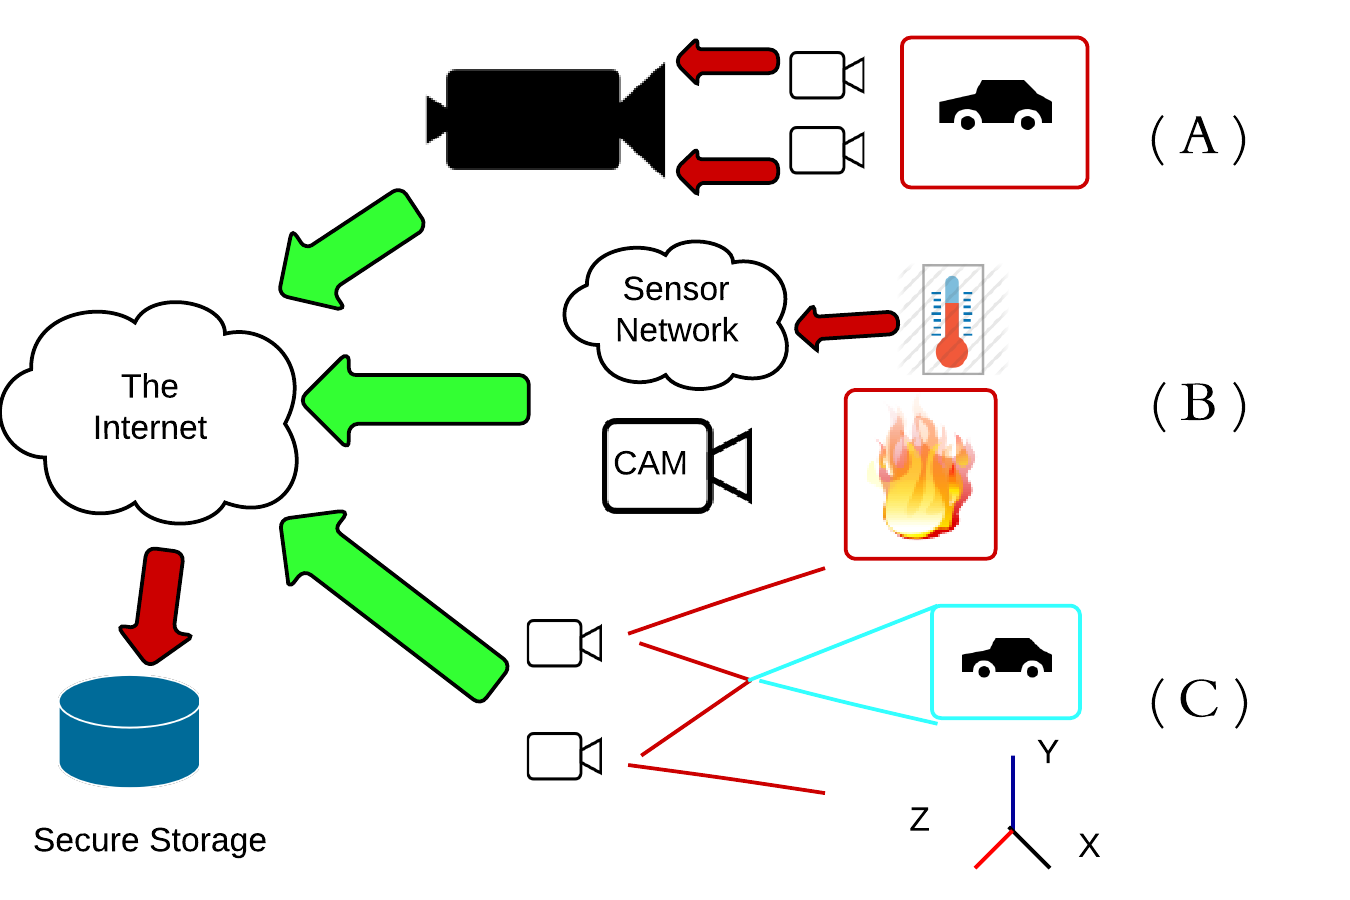
\includegraphics[scale=0.3]{CameraDepolymentsFigure.png}
\caption{\textbf{(A)} Shows a multi-tier smart camera network in which more efficient low cost camera do object detection and wake up higher resolution cameras to run computer
vision algorithms. \textbf{(B)} Is an example of sensor fusion where non-image sensing networks can use its data with the video data to make a better evaluation of the situation.
\textbf{(C)} An object being detected by redundant coverage can be given a position in three dimensional space for computer vision algorithms to use.}
\end{figure*}

\section{Wireless Smart Camera Surveillance}
Researchers and Commercial companies are designing wireless smart camera networks in surveillance applications to prevent crimes, detect environmental emergencies,
monitor behavior of the elderly, and track vehicular traffic in public spaces. Many camera platforms have been designed to meet strict hardware requirements~\cite{Flexi-WVSNP}~\cite{Citric}~\cite{WiFLIP} for wireless deployment in surveillance systems. However, different requirements must be stated when looking at the application specific 
scenario of surveillance in public spaces. To understand how these state of the art systems are improving on designs of the past, one must define what makes these
surveillance systems "smart". These smart camera network systems have common goals when it comes creating more efficient surveillance applications. First, the issue 
of network resource utilization is an issue all systems need to consider if those surveillance systems are to be scalable in crowded wireless deployment 
scenarios. Then in almost every application considering power consumption of each node is very important if one is give an analysis of the systems 
efficiency. If these systems are to be monitoring public spaces the smart camera networks need to be keeping the data recorded secure and also
ensuring that the data recorded is actually quality information that could be used by officials. 

\subsection{Bandwidth Efficiency}
Video data is rich with useful information that other sensor sources can’t provide, however video data quickly becomes very large in size as time goes 
on.Nodes competing for network connectivity while maintaining quality on live video feed can soon become a problem as the network grows or if other 
nodes not in the system share the connection. One way to combat this is by assuring the data recorded is useful and actually recording video data that 
can be used to do detection of events by doing in network processing ~\cite{Citric}.\\

Taking advantage of multiple cameras is a very useful method to determine not only which node has the best view of the object, but also if the overlapping
video footage can be combined to provide more useful data. Extensive research has been done on both bandwidth and energy efficiencies of wireless
smart camera networks that make use of overlapping footage ~\cite{AccLatEnergy}.


\subsection{Lowering Power Consumption}
 When discussing wireless sensor networks , power consumption is always brought up as a concern in deployment and scalability. Smart camera networks are 
no different, and many researchers have discussed methods to design nodes that consume less power. One such method would be to limit the amount of time 
a camera needs to actually be powered on, and rely on more low power sensors to trigger a wake up. Using this sensor fusing technique allows the system
to operate a different power consumption states . Such states must be carefully looked at and many researchers 
consider every level of operation of each camera node ~\cite{AccLatEnergy}~\cite{EnergyCons}. Making Smart hardware choices, such at choosing low power communication
options such as 802.15.4, can also have a large effect on how much power the system uses.

\subsection{Quality of data recorded}
Vision sensor data requires much higher bandwidth due to its two-dimensional nature of its pixel arrays, and such data can not be fully analyzed by humans~\cite{MeshEye}.
Recording live high-resolution data all the time with no inference will soon become a thing of the past. Every second of video recorded counts when the 
surveillance system scales to much larger deployments such as in smart cities~\cite{HuSIMS}. Doing local processing and decision making first can have 
a huge change on the amount of data that actually needs to be transmitted and archived. Whether it is event detection or object identification, preventing 
false alarms by checking the data locally can be very helpful. The research area of computer vision has grown at a very fast rate and only in the past few years
are we seeing wireless surveillance systems adopt these sophisticated algorithms.

\section{Smart Camera Advantages}

Researchers are using common design strategies to overcome chalanges when using smart camera networks for surveillance. From deployment strategies to choosing efficient
hardware and software, researchers are making wireless surveillance systems smarter. Before presenting our taxonomy of current research systems, we will define
some terminology and present some generic concepts.


\subsection{Efficiency in Smart Camera Networks}
Measuring performance in a wireless smart camera networks can be broken up into 2 specific categories. One having to do when environmental impact of these systems its important
to measure how much energy these monitoring systems use on a daily basis. Many strategies from other wireless sensor networks can be used in this scenario including
making use of nodes that sleep during idle times. Another technique is to use hardware that uses less power to decide if it needs to wake the more power hungry video sensors.


A few solutions to both performance concerns show up in many systems design by researchers today. As shown in Figure 1, smaller more energy and bandwidth efficient sensor networks
could provide smaller meta data such and audio and temperature data to complement what the video sensor captures. When Computers analyze both data sets and
make an inference about them its called sensor fusion or multi-modal sensor networks. Designing the vision sensor network to take advantage of two classes of cameras, one 
efficient and the other more powerful and higher resolution, also helps with performance. Deciding on a smart deployment strategy can also be very beneficial,
especially in scenarios with overlapping coverage. Getting multiple views of an object get give more data and much more accuracies.

\subsection{Implementation strategies}
An important decision made when designing smart camera platforms is what communication medium will be chosen. Many systems choose Zigbee(802.15.4) as their wireless 
communication link for its low power features, whereas if your system has a higher bandwidth requirement researchers choose the more ubiquitous WiFi(802.11). The camera platforms
and monitoring systems software architecture must also be analyzed when classifying effectiveness in the application of surveillance. Classifying the systems security mechanism 
to both secure the data and also its transmission channels.  

\subsection{Common Computer Vision Techniques}

\subsubsection{Object Detection and Recognition}
One the objectives of the computer vision and the image processing, is the ability of identify and classify instances of real-world objects in images or videos.
It has been developed different algorithms with different approaches to this same problem. There are 2 main used techniques for object detection, one based on 
training the objects to be detected and recognized, while the other is based on detecting moving objects using background subtraction and recognize 
them through the shape.

\subsubsection{Behavior Tracking}
An area is emerging in the surveillance systems, algorithms capable of tracking the human behaviour to better categorize the data being recorded. The use of 
this kind of system can automate the process of analysing the human movements and, from there, identify abnormal behaviors and hostile intent  that can be 
translated as alerts for the system supervisors.

\subsubsection{Occlusion Handle}
Surveillance cameras are usually developed to work independent of the ambient. Therefore, scenarios that have many obstacles that can occlude the vision of 
the camera over the detected object can represent a problem. In order to increase the tracking capability of the systems, some of them have an additional 
component responsible for the occlusion handle, in other words, the system is able to track the object even if it cross by another moving or static object.

\begin{table*}[t]
  \centering

  \begin{tabular}{| p{1.1cm} | p{2cm} | p{1.2cm}  | p{2.1cm} | p{1cm} | p{2.5cm} | p{1.5cm} | p{1.3cm}  | p{2cm} |}
    \hline
    System & Energy Efficiency & Multimodal & Bandwidth Efficiency & Wireless & Video Analysis & System Software & Multicamera Overlap & Security \\   \hline
    
    Citric & sleeping nodes, only wake on presence of objects & Audio & In-network image processing, small image size & 802.15.4
     	& \textbf{Compression:} Compressed Sensing, \textbf{Object Detection:} Frame Differencing Background Subtraction, \textbf{OcclusionHandle:} Multiple Cameras For One Object 
        & Embedded Linux & Yes & Pre-processing of data at node, wireless protocols \\ \hline
    
    HuSIMS & small processing power cameras, power efficient sensors & Smoke detectors, motion, light, humidity, Temperature 
    	& In-network image processing, Sink nodes, separate low bandwidth sensor networks  
    	& WiMAX 4G & \textbf{Alerts:} Object Abnormal Behavior & Large Management Software using semantic processing 
    	& No & given by 4g and secured at control center  \\ \hline
    
    OmniEye & none described for cameras, seperate energy efficient sensor network & temperature light, sound sensors 
    	& In-network image processing, data annotation 
    	& 	WiPort 802.11b/g TSAM MAC & \textbf{Compression:} JPEG 70\% ,   \textbf{Object Detection:} Adaptive Background Subtraction 
        & \textit{u}Linux & Yes & Data encrypted using PICO, SSL communication  \\ \hline
    
    Wi-FLIP & analog circuitry, low-level image processing, smart image processor & Light & Small images, Low framerate  
    	& 802.15.4 & \textbf{Object Detection:} Difference of Gaussians  & TinyOS & No & none described  \\ \hline
    
    SensEye & multi-tier cameras, cameras sleep because of redundant coverage  & none & low-latency wakeups and detection  
    	& 802.11,  900MHz  & \textbf{Object Detection:} Frame Differencing Background Subtraction, \textbf{OcclusionHandle:} Multiple Cameras For One Object  
        & Embedded Linux & Yes & wireless protocols  \\ \hline
    
    DTN-Citric & sleeping nodes, only wake on presence of objects & Audio & Distributed In-network processing, In-network storage  & 802.15.4 
    	& \textbf{Object Detection:} Not Specified Background Subtraction & Embedded Linux  & Yes & Encrypted network traffic  \\ \hline
    
    Flexi-WVSNP & switching between radios, efficient SoC processor & Zigbee sensor network  & switching between radio's to control channel utilization  
    	& 802.11, 802.15.4 & None Described & Custom SoC Firmware & No & None described  \\ \hline
    
    MeshEye & Low powered transievers, designed for battery power & none & Distributed in-network processing   & 802.15.4 
    	& \textbf{Object Detection:} Frame Differencing Background Subtraction & Custom Arm7 microcontroller firmware & No & None Described  \\ \hline


  \end{tabular}
  \caption{}{A taxonomy of current research surveillance systems that use wireless smart cameras}
  \label{tab:1}
\end{table*}



\section{Classifying Smart Wireless Surveillance Systems}

\subsection{Energy Efficiency}
All of the systems listed in Table 1 make an effort to reduce power consumption their system in some way. Getting the system to go into a low powered 
sleep state during idle periods is a very effective solution ~\cite{AccLatEnergy} ~\cite{Citric}. Non-image sensors are already extremely energy efficient, 
there for its often useful to use them to determine when the system should turn on the power hungry camera nodes. The image sensor itself can be design with
analog circuitry and be more compact which will also reduce energy consumption~\cite{WiFLIP}. However the lower power consumption comes at a cost, and with
the Wi-FLIP camera platform its frame rate.In surveillance systems with redundant coverage, which we discuss later, camera nodes can also tell their neighbor
nodes to turn on or off based on the tracked object's trajectory in the scene~\cite{SensEye}.Efficient SoC processor are now more advance and can handle
managing a smart camera node while being energy efficient~\cite{Flexi-WVSNP}.

\subsection{Sensor Fusion}
Using multiple sensors can also allow you to create more specific alarms cases that tell you more than just that an event occurred. The Human Situation
Monitoring System does this on a very large scale by using numerous sensors is dense city deployments ~\cite{HuSIMS}. Sensors may be on the wireless camera
node on may be on its own sensor network as in the OmniEye system ~\cite{OmniEye}. The extra sensors don't necessarily need to be non-image sensor but 
could in fact be low powered camera sensors for simpler sensing tasks that then trigger larger more powerful cameras to be activated~\cite{SensEye}.

\subsection{Network Load and Scalability}
With high resolution streams coming from each of the camera nodes in these surveillance systems, it becomes impossible to have 
that much video data be transmitted at once. Many systems take advantage of in-network processing before sending the data out to the internet or do processing on
the wireless camera node itself ~\cite{HuSIMS}~\cite{OmniEye}. By annotating important data that displays and event of interest, system managers can request smaller sets 
of data based on meta data~\cite{OmniEye}. Making use of sink nodes in densely populated sensor networks is also a very popular technique to reduce the 
amount of rich video data needs to be sent over the internet~\cite{HuSIMS}. Another important factor to consider when discussing network load is channel utilization,
minimizing time spent on one wireless communication by sending data on another also helps in network load efficiences~\cite{Flexi-WVSNP}.


\subsection{Wireless Communication}
If the surveillance system is densely populated and would cause to great a load on nearby networks, options such at WiMAX may be used ~\cite{HuSIMS}. 
Researchers working on the OmniEye project and MeshEye project have even design their own MAC layer protocols to scale better in larger topologies ~\cite{MeshEye}~\cite{OmniEye}. In surveillance 
situations where wireless communication is intermittent , delay tolerant networking techniques may be used ~\cite{DTNSmartCamera}. In DTN based systems, data
may be allowed to accumulate locally before being transmitted securely over the internet. Systems may have a hybrid communication system, where they take advantage of
two seperate radios~\cite{Flexi-WVSNP}. Doing this could reduce the amount of traffic produced by the node to any of the 2 radio communication links.


\subsection{Computer Vision in Surveillance}
As already said, it would be very helpful if all the captured images could be analysed in the node before being uploaded and saved. Most of the systems that use in node
data process are using background subtraction method to detect moving objects with single cameras in real-time. There are different algorithms to implement it, with 
different computer efficiencies and accuracies, what can make each one more suitable for each system.

\subsubsection{Object Detection and Recognition}
Methods like Mixture of Gaussians (MoG) ~\cite{CS-MoG} or frame differencing, sometimes with adaptive background, are largely used ~\cite{OmniEye}~\cite{SensEye}~\cite{MeshEye}, but 
the computational efficiency still a problem. In Johnsen and Tews ~\cite{Occlusion}. it is shown the possibility of having a low power and computationally efficient 
(up to 5 times faster) system based on  background subtraction using a very known method: Compressed Sensing. Using CS is possible to compress the image, in other words, reduce 
the amount of data to be processed, while retaining much of the original image. The compressed image can be submitted to a MoG algorithm to detect the objects on the scene with 
a lower solution complexity. The results shown a very efficient system, that they called CS-MoG, with an accuracy very close to a system that uses MoG only.

The CITRIC ~\cite{Citric} system resembles Johnsen and Tews ~\cite{Occlusion}. by the steps that are used in the object detection. At first they use CS to compress the image, 
then they use frame differencing to do background subtraction and apply Canny edge detection algorithm to detect the objects. On their most recent work, they describe a new 
method called Distributed Object Recognition, where they try to boost the recognition accuracy using multiple cameras to recognize the same object. Motivated by the CS and its
applications in sensor networks, they show that the visual histogram of the features that describe an object in a single image is spare, and most of its coefficients are positive
and approximately zero. Furthermore, since SIFT-type features (e.g., SIFT [Lowe 1999], SURF [Bay et al. 2008], or CHoG [Chandrasekhar et al. 2009]) are robust to some degree of 
camera rotation and translation, it is possible to relate the non zero coefficients of the features from one camera with the others from other cameras. This phenomenon is called 
joint sparsity (JS).

\subsubsection{Behavior Tracking}
On the HuSIMS system ~\cite{HuSIMS} they take one step further after tracking the objects, it is implemented an algorithm that is able to trigger alarms if something looks
irregular. Afterdoing the object tracking they are able to define regions, representing where the most common tracks pass by, and sinks, representing places where the objects
usually appear or disappear from the scene. Having these 2 defined sections there is an algorithm capable of analysing the image and verify, for example, if the objects of a
certain type is following the expected region for its type, or if the object went from one sink to another. In a case where one of these predicted behaviours looks different,
an alarm is triggered notifying that a problem could happened.

\subsubsection{Occlusion Handle}
A problem very common with single camera systems is the object occlusions. A good method for this case is presented in [8 check]. After a background subtraction they are 
classified accordingly to the change of their shape through the time. It is used a Kalman filter to predict the position of the objects and then compare the current position
with the predicted one through an algorithm that allows the system to even distinguish between a single person or a group of people as seen on Figure 2 The particular 
characteristic of this algorithm is the ability to track objects with complete occlusion for a long duration.

\begin{figure}[h!]
\centering
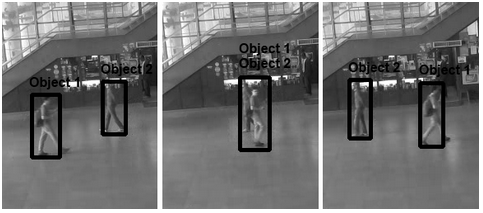
\includegraphics[scale=0.5]{Occlusion.png}
\caption{Occlusion handle algorithm as described by Swantje Johnsen and Ashley Tews ~\cite{Occlusion}.}
\end{figure}	

Others occlusion handle methods can be used. On HuSIMS  ~\cite{HuSIMS} , a less accurate, but also less complex, detects the edges along which a target disappears and then fits
lines. Another example is CITRIC ~\cite{Citric}, where they take the advantage of multiple cameras and the distributed recognition to keep the track of an object even after 
the object become occluded for one of the cameras.


\subsection{Management Software}
At the wireless camera  node level there are two clear options when it comes to operations systems, one either chooses an smaller architecture for 
simplicity or one that can do on node processing and run more complicated analysis tools.
It is well known that monitoring many feeds at once is very hard to automated and just does not scale well. Therefor some researchers are using semantic
interpretation to abstract the raw data into more generic anomalies ~\cite{HuSIMS}. 

\subsection{Overlapping Multi-camera Advantages}
The Citric project designed their camera node to incorporate redundant coverage into their video analysis, and can track and object in 3 dimensional space if the object
is found in the view of two cameras~\cite{OmniEye}~\cite{DTNSmartCamera}.The Citric platform is not the only system that when deployed makes use of overlapping video data. 
Not only are the cameras over lapping in the SensEye system, but their two levels of complexity because of their multi-tiered camera setup~\cite{SensEye}.

\subsection{Securing The Data}
Privacy is a major concern is the design process of today's wireless sensor networks. Systems need to secure the private data that has been processed, the
transmission link, and to location at which the data is stored. Many systems choose to rely on the standard methods provided by the technologies they use
~\cite{HuSIMS}. While others make use of sophisticated encryption tools to secure its data and more commonly known secure communication tools such as Secure
Socket Layer(SSL) ~\cite{OmniEye}. Wireless Surveillance systems must protect any data that could leak private information about objects and environments they track to those
sniffing the communication medium. 

\section{The SWEETcam Project}
As a proof of concept we've designed our own wireless smart camera node to help improve safety on campus. we've made use of the very popular RaspberryPi for
its powerful processing capabilities, low cost, and its capability to run Linux. Some components we found very useful to achieve our goals including the 
Broadcom SOC(System On a Chip), 700 MHz ARM processor, and its very own GPU for video processing. With the system running Linux, it was very easy for us to
make use of many computer vision libraries already developed for Linux systems.\\
We developed using the newly released Raspberry Pi camera module, which has an available API in C language and is capable of capturing 1920x1080 resolution
color images with 30 fps rate. For the image processing, we chose the Open Source Computer Vision Library (OpenCv). Our computer vision system is developed in 
C++ for better integration between the OpenCV and the API.

\subsection{Project overview}

\-- show both software and hardware diagram

\subsection{Energy Harvesting}
Researchers agree that one way to combat the problems of lifetime performance with battery powered wireless sensor nodes is by making use of energy-harvesting
capabilities~\cite{EnergyHarvesting}. We plan on achieving this with our system by using current solar technologies to recharge the camera's local battery. 
Doing this we hope our system will require much less maintanence and remove any requirements for node placement near power grids.

\subsection{Image Processing}
\- Considering the constraints of the system in terms of price and hardware, it is used techniques of background subtraction to do the object detection.
When started, the program keep taking pictures and process them using Mixture of Gaussian (MoG) method by Stauffer and Grimson. With the foreground in
hands we find the contours and then a bounded box is applied following the contours' limit. To remove some noise and false detection a step is added to 
ignore objects of small size. The object classification is the most processor consumption  processes for most of the pedestrian detection systems, 
because it is used training techniques to classify the objects based on a previous stored database. In our case, to reduce the process we classify the 
objects by looking at their dimensions, they are classified as human if the height is two times bigger than the width we classify as a person. \\
\begin{figure}[h!]
\centering
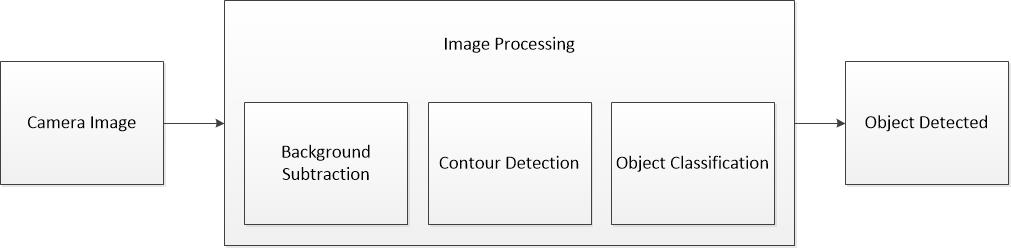
\includegraphics[scale=0.3]{imageprocessing.jpg}
\end{figure}	
\- This light system can generate some false alarms, but in association with the whole system, and its sensors, it can be improved for a better
performance. There are other more robust object detection methods that could be used, but we would have a very low fps rate. 

\subsection{Tracking Object Behavior}
Researchers in the computer vision  field are now moving to not only detect objects and their movements, but to then infer a given behavior is being displayed.
Looking for patterns in the way objects move will help us make better assumptions about what those objects are doing at a more generic level. Using this
information we can do better event detection for specific occurrences and tag the video recorded accordingly. For example, video data that specifically states
it is a recording of a person by a bike rack late in the evening is much more useful that video recorded of just a person.


\section{Future Directions and Lessons to take away}
Many Embedded systems can apply the same classification we present here to their systems as well. Such systems become more numerous every day and therefor their
footprint on both the amount of energy they consume and the load they add to today's Internet is important. For such architectures to remain scalable,
future monitoring system will need to be more self reliant which includes having decision making and data processing be done from within the system itself.
Much research still remains to achieve this goal in smart camera networks for surveillance and other sensor networks and systems.



%% *************************  END PAPER **********************************


% Can use something like this to put references on a page
% by themselves when using endfloat and the captionsoff option.
%\ifCLASSOPTIONcaptionsoff
%  \newpage
%\fi


%% ******************  REFERENCE SECTION **********************************

\bibliography{Bib.bib}{}
\bibliographystyle{plain}


%% ******************  AUTHOR BIOGRAPHIES *********************************

\begin{IEEEbiographynophoto}{Kevin Abas}
is a graduate student at Univeristy of California Santa Cruz. His research
interests include wireless sensor networks, computer networking, and embedded
systems. He recieved his BSc in computer engineering from University of
California Santa Cruz. Contact him at kabas@soe.ucsc.edu.
\end{IEEEbiographynophoto}

\begin{IEEEbiographynophoto}{Caio Porto}
Biography text here.
\end{IEEEbiographynophoto}

\begin{IEEEbiographynophoto}{Katia Obraczka}
Biography text here.
\end{IEEEbiographynophoto}

\end{document}

%%------------------------------------------------------------------------

